% Provenance (never printed): see sources/outline_sources.md (Year 3:
% radial velocity, transits, imaging and microlensing; what has been
% found; atmospheres from transmission spectra).
% Brief: sources/book5/BRIEFS.md, ch. 28. Curves from figdata/bachelor-3/
% rv_transit.py (Keplerian radial-velocity curves, a limb-darkened transit
% light curve computed by numerical integration, point-lens microlensing)
% and exoplanet_archive.py (the NASA Exoplanet Archive's composite table of
% confirmed planets, fetched 2026-10-23, with the model mass--radius curves
% of Zeng et al.). Exercise and problem values in the Book 5 scratch
% calculator calc/ch28.py. Selene's Lamp and its planet are invented.
\chapter{الكواكب الخارجية}\label{ch:b3:exoplanets}

في خريف عام 1994، قاس فلكيّان سرعات 142
نجمًا فوجدا أنّ أحدها، 51~بيغاسي، يتحرّك نحونا ويبتعد عنّا
بدورٍ قدره نحو أربعة أيّام. بلغ نصف سعة الحركة
\qty{59}{m.s^{-1}}، أي أربعة أضعاف ما كان مطيافهما قادرًا على كشفه.
كان الرفيق الذي يجرّ النجم في مداره يملك كتلة لا تقلّ عن نصف كتلة
المشتري، على مدار بُعده \qty{0.05}{au}، أي أقرب إلى نجمه ثماني مرّات
من بُعد عطارد عن الشمس. لم يكن لأيّ نظرية في تكوين الكواكب مكانٌ
لمثل هذا الجرم. أُعلن الاكتشاف في أكتوبر 1995 فافتتح مجالًا جديدًا في علم الفلك:
بعد ثلاثة عقود، تأكّد وجود أكثر من ستّة آلاف كوكب تدور حول
نجوم أخرى، ورُصد بعضها مباشرةً،
وحُلّل الغلاف الجوي لبعضها. يعرض هذا الفصل كيف تُكتشف الكواكب الخافتة
التي لا تُرى بالعين، وما الذي تمّ العثور عليه، وكيف تُقرأ
أغلفتها الجوية.
% ledger: nobel19:51peg, planet:Mercury.dist, data:b5-pscomp

\begin{recall}
تأثير دوبلر، والسرعة الشعاعية، والثنائيات الطيفية، وقوانين كبلر،
ومسألة الجسمين ومركز كتلتهما، وقانون بلانك،
والارتفاع المقياسي لغلاف جوي متساوي الحرارة تَرِد في كتب الفيزياء.
والكوكب الخارجي والنطاق الصالح للحياة لنجم ما يَرِدان في كتب المدرسة.
الدفق والإشعاعية لمصدرٍ ما يَرِدان في مجلد السنة الأولى، في فصلها
عن التلسكوبات والقياس الضوئي؛ ودرجة الحرارة التوازنية في فصلها
عن علم الكواكب المقارن. يَرِد تكوين الكواكب وخطّ الثلج في مجلد السنة الثانية.
\omterm{def:b3:planetary-atmospheres:jeans-escape}{وإفلات جينز}، \omterm{def:b3:planetary-atmospheres:hydrodynamic}{والإفلات الهيدروديناميكي}، وحدود
النطاق الصالح للحياة تَرِد في هذا المجلد، في فصلها عن الغلاف
الجوي للكواكب.
\end{recall}

\section{طريقة السرعة الشعاعية}\label{sec:b3:exoplanets:rv}

لا يدور الكوكب حول نجمه: فكلاهما يدور حول مركز كتلتهما المشترك.
والنجم، وهو أثقل بكثير، يتحرّك على مدار صغير خاص به، ويُزاح ضوؤه
بتأثير دوبلر ذهابًا وإيابًا بدورة الكوكب.

\begin{definition}[طريقة السرعة الشعاعية؛ الكتلة الدنيا]\label{def:b3:exoplanets:rv}
\emph{طريقة السرعة الشعاعية}\index{طريقة السرعة الشعاعية} تكشف كوكبًا
عن طريق التغيّر الدوري للسرعة الشعاعية لنجمه،
المقاسة من إزاحة دوبلر لخطوط طيف النجم. وحين
يكون ميل المدار $i$ على مستوى السماء مجهولًا، فإنّ الطريقة
لا تقيس إلّا الجداء $m_p\sin i$ أي كتلة الكوكب مضروبةً في جيب
الميل، أي \emph{الكتلة الدنيا}\index{الكتلة الدنيا}
للكوكب.
\end{definition}

\begin{theorem}[نصف سعة السرعة الشعاعية]\label{thm:b3:exoplanets:semi-amplitude}
ليكن نجمٌ كتلته $M_\star$ وكوكبٌ كتلته $m_p$ على مدار دائريّ
دورُه $P$، مائلًا بزاوية $i$، ويُعطي النجمَ سرعةً شعاعية
$v_r(t) = \gamma + K\cos\bigl(2\pi(t - t_0)/P\bigr)$، حيث $\gamma$ هي
سرعة مركز الكتلة، ونصف السعة
\[
K = \left(\frac{2\pi G}{P}\right)^{1/3}
    \frac{m_p\sin i}{(M_\star + m_p)^{2/3}} .
\]
على مدار لامركزيّته $e$، لم يعُد المنحنى جيبيًّا،
$v_r = \gamma + K\bigl[\cos(\nu + \omega) + e\cos\omega\bigr]$، حيث $\nu$
الشذوذ الحقيقي و$\omega$ زاوية الحضيض، وتُقسم $K$
على $\sqrt{1 - e^2}$.
\end{theorem}

\begin{proof}
في حالة المدار الدائري: يخضع البُعد $a$ بين الجسمين
لقانون كبلر الثالث، $a^3 = G(M_\star + m_p)P^2/4\pi^2$. ويقع النجم على
بُعد $a_\star = a\,m_p/(M_\star + m_p)$ عن مركز الكتلة،
ويقطع دائرته بسرعة $v_\star = 2\pi a_\star/P$. ومنه
\[
v_\star = \frac{2\pi}{P}\,\frac{m_p}{M_\star + m_p}
          \left(\frac{G(M_\star + m_p)P^2}{4\pi^2}\right)^{1/3}
        = \left(\frac{2\pi G}{P}\right)^{1/3}\frac{m_p}{(M_\star + m_p)^{2/3}} .
\]
يصنع خط النظر الزاوية $\pi/2 - i$ مع مستوى
المدار، فلا يقع على الخط إلّا $v_\star\sin i$ من سرعة النجم،
وتلك المركّبة تدور مع النجم: $v_r - \gamma = v_\star\sin i\,
\cos\bigl(2\pi(t - t_0)/P\bigr)$. ويُستنتج الشكل اللامركزي من
القطع الناقص الكبلري، ويُسلَّم به.
\end{proof}

ولمّا كان الكوكب أخفّ بكثير من نجمه، فإنّ $K$ يحدّد $m_p\sin i$
بعد قياس الدور ومعرفة كتلة النجم من
طيفه. فبالنسبة إلى 51~بيغاسي~b، حيث $K = \qty{59}{m.s^{-1}}$ و$P = \qty{4.23}{d}$
حول نجم كتلته شمسٌ واحدة نحصل على $m_p\sin i = 0.47$ من كتلة المشتري.
يُحرّك المشتري الشمسَ بسرعة \qty{12.5}{m.s^{-1}} خلال مداره البالغ \num{4331} يومًا
ولو رصد راصدٌ بعيدٌ سرعة الشمس لوجدها تتأرجح بنحو
\qty{\pm 13}{m.s^{-1}} خلال اثنتي عشرة سنة. وتُحرّك الأرض الشمسَ بسرعة
\qty{9}{cm.s^{-1}}. والمطياف الذي اكتشف 51~بيغاسي~b بلغ
\qty{13}{m.s^{-1}}؛ وتبلغ خلائفه نحو \qty{1}{m.s^{-1}} (أي
سرعة المشي \qty{3.5}{km/h})، والأحدث منها مُصمَّم لبلوغ نحو
\qty{10}{cm.s^{-1}}، ويكفي لكوكب بكتلة الأرض في النطاق الصالح للحياة
حول نجمٍ منخفض الكتلة، حيث يكون مدار الكوكب قصيرًا ونجمه خفيفًا.
ويضع النجم نفسه حدًّا أدنى: فالنبضات والبقع على سطحه،
التي يحملها دورانه، تُزيح خطوطه أيضًا، ويجب أن تُميَّز إشارة الكوكب
عنها.
% ledger: nobel19:51peg, nobel19:sun-jupiter, nobel19:migration, planet:Jupiter.mass, planet:Jupiter.Porb, planet:Jupiter.ecc, planet:Earth.mass, sun:mass, eso:espresso, const:G

\begin{omfigure}
\centering
\begin{tikzpicture}
\begin{axis}[width=0.86\linewidth, height=0.40\linewidth,
  xmin=0, xmax=2, ymin=-40, ymax=42,
  xlabel={الطور المداري (بالدورات)}, ylabel={\mbox{\textdir TLT $v_r - \gamma$ (\unit{m.s^{-1}})}},
  tick label style={font=\scriptsize}, label style={font=\small},
  legend style={font=\scriptsize, at={(0.5,-0.30)}, anchor=north, legend columns=2, draw=none, cells={anchor=west}, /tikz/every even column/.append style={column sep=1em}}]
\addplot[thin, black!40, forget plot] coordinates {(0,0) (2,0)};
\addplot[thick, omDef] table[x=phase, y=v_circ] {figdata/out/bachelor-3-rv_transit-rv.dat};
\addlegendentry{مدار دائري}
\addplot[thick, dashed, red!70!black] table[x=phase, y=v_ecc] {figdata/out/bachelor-3-rv_transit-rv.dat};
\addlegendentry{{\foreignlanguage{arabic}{مدار لامركزي، $e = 0.3$، }}\mbox{\textdir TLT $\omega = \ang{60}$}}
\draw[<->, thick] (axis cs:1.0,0) -- (axis cs:1.0,30);
\node[font=\scriptsize, anchor=east] at (axis cs:0.99,12) {$K$};
\end{axis}
\end{tikzpicture}
\par\smallskip{\small السرعة الشعاعية لنجم يضمّ كوكبًا واحدًا، على مدى
دورتين مداريّتين، لكوكب مُتخيَّل بقيمة $K = \qty{30}{m.s^{-1}}$ ودور
قدره عشرة أيّام. في مدار دائري (متصل) يكون المنحنى جيبًا
نصف سعته $K$. وفي مدار لامركزي (متقطّع) يتحرّك النجم
أسرع ما يكون قرب الحضيض، فيصير المنحنى مائلًا: قيمتا قصواه هما
$K(1 \pm e\cos\omega)$، ويبقى المدى من القمة إلى القاع
$2K$.}\label{fig:b3:exoplanets:rv}
\end{omfigure}

\section{العبورات}\label{sec:b3:exoplanets:transits}

إذا رُئي المدار تقريبًا على حافّته،
يمرّ الكوكب أمام نجمه مرّةً في كلّ دورة، فيحجب جزءًا صغيرًا من قرصه.

\begin{definition}[طريقة العبور؛ عمق العبور؛ معامل التصادم]\label{def:b3:exoplanets:transit}
تكشف \emph{طريقة العبور}\index{طريقة العبور} الكوكبَ من خلال
الخفوت الدوري لنجمه عندما يعبر الكوكب قرص النجم. ويُمثّل
\emph{عمق العبور}\index{عمق العبور} $\delta$ الانخفاضَ الكسريّ
للدفق النجمي أثناء العبور. ويُمثّل \emph{معامل
التصادم}\index{معامل التصادم (العبور)} $b = a\cos i/R_\star$ أصغرَ المسافات
بين مركزي الكوكب والنجم كما تُرى في السماء،
مقيسةً بوحدات نصف قطر النجم $R_\star$، لمدار نصف قطره $a$
وميله $i$.
\end{definition}

\begin{proposition}[عمق العبور]\label{prop:b3:exoplanets:depth}
يُعطي كوكبٌ معتم نصف قطره $R_p$ يقع كليًّا أمام نجم ذي سطوع منتظم
العمقَ $\delta = (R_p/R_\star)^2$.
\end{proposition}

\begin{proof}
يحجب الكوكب المساحةَ $\pi R_p^2$ من قرص مساحته $\pi R_\star^2$
الذي يتساوى سطوعه في كلّ موضع؛ فينخفض الدفق بالنسبة ذاتها.
\end{proof}

لو عبر المشتري الشمسَ لخفتت بمقدار \qty{1.06}{\percent}، ولو عبرتها الأرض
بمقدار \num{84} جزءًا في المليون؛ فالأول في متناول
تلسكوب صغير، أمّا الثاني فيحتاج إلى تلسكوب فضائي يقيس آلاف
النجوم سنواتٍ عدّة. غير أنّ القرص النجمي ليس منتظمًا.

\begin{definition}[إعتام الحافة]\label{def:b3:exoplanets:limb}
\emph{إعتام الحافة}\index{إعتام الحافة} هو تناقص السطوع السطحي
للنجم من مركز قرصه إلى طرفه، أي الحافة.
قرب الحافة يدخل خط النظر غلافَ النجم الجوي مائلًا،
ويبلغ العمق البصري الواحد في طبقات أعلى وأبرد، وهي تُشعّ
قدرًا أقلّ. ويُكتب غالبًا قانونًا تربيعيًّا بدلالة $\mu = \cos\theta =
\sqrt{1 - r^2}$، حيث $r$ البعدُ عن مركز القرص مقيسًا
بوحدات أنصاف أقطار النجم: $I(\mu)/I(1) = 1 - u_1(1 - \mu) - u_2(1 - \mu)^2$.
\end{definition}

يحجب الكوكبُ القريب من مركز قرص معتم الحافة ضوءًا أشدّ سطوعًا
من المتوسّط ويعمّق العبورَ؛ وقرب الحافة يحجب ضوءًا أقلّ.
قاعُ منحنى الضوء مستدير، وتلين حوافّه. وتحمل مدّةُ
العبور معلوماتٍ عن هندسة المدار.

\begin{theorem}[مدّة العبور]\label{thm:b3:exoplanets:duration}
في مدار دائري دوره $P$ ونصف قطره $a$ وميله $i$، ولنأخذ
$p = R_p/R_\star$ \omterm{def:b3:exoplanets:transit}{ومعامل التصادم} $b$، فإنّ الزمن من التماسّ الأول
إلى الأخير هو:
\[
T_{14} = \frac{P}{\pi}\arcsin\!\left(\frac{R_\star}{a}\,
          \frac{\sqrt{(1 + p)^2 - b^2}}{\sin i}\right),
\]
ويُعطى الزمن بين التماسّين الثاني والثالث، حين يكون الكوكب
بكامله داخل القرص، وهو $T_{23}$، بالصيغة نفسها مع
$1 - p$ بدلًا من $1 + p$.
\end{theorem}

\begin{proof}
لتكن $\varphi = 2\pi t/P$ الطورَ المداري مقيسًا من منتصف العبور.
إسقاطًا على السماء، حيث $x$ على طول مسار الكوكب و$y$ عموديًّا عليه،
يقع مركز الكوكب عند $x = a\sin\varphi$ و$y = a\cos i\cos\varphi$
عن مركز النجم. وبوحدات نصف قطر النجم، يكون مربّع البعد هو:
\[
z^2 = \left(\frac{a}{R_\star}\right)^2(\sin^2\varphi + \cos^2 i\cos^2\varphi)
    = \left(\frac{a}{R_\star}\right)^2\sin^2 i\,\sin^2\varphi + b^2 .
\]
يتماسّ القرصان من الخارج عندما $z = 1 + p$، عند
$\sin\varphi = \sqrt{(1 + p)^2 - b^2}\,R_\star/(a\sin i)$، متماثلًا
حول منتصف العبور. ويستغرق العبورُ الطورَ $2\varphi$، أي الزمنَ
$2\varphi P/2\pi = P\varphi/\pi$. وعند $z = 1 - p$ يتماسّ القرصان
من الداخل.
\end{proof}

في المدار الواسع يُقرَّب الجيب العكسي بحجّته: $T_{14} \approx (P/\pi)
(R_\star/a)\sqrt{(1 + p)^2 - b^2}$. أطول العبورات ما كان مركزيًّا؛ أما
عبورُ الحافّة، حين يكون $b$ قريبًا من $1 + p$، قصيرًا على شكل حرف V. ويفضي قياس
$T_{14}$ و$T_{23}$ على منحنى الضوء إلى $b$ و$a/R_\star$، ومنهما
الميلُ: فالعبور يزيل $\sin i$ الذي تتركه السرعة الشعاعية
مجهولًا.

\begin{omfigure}
\centering
\begin{tikzpicture}[scale=0.92]
\shade[inner color=yellow!25, outer color=orange!70] (0,0) circle (2);
\draw[orange!70!black] (0,0) circle (2);
\draw[dashed, black!60] (-3.2,-0.6) -- (3.2,-0.6);
\draw[->, black!60] (2.5,-0.6) -- (3.2,-0.6) node[right, font=\scriptsize] {مسار};
\foreach \x in {-2.117, -1.697, 1.697, 2.117} {\fill[black] (\x,-0.6) circle (0.2);}
\node[font=\scriptsize] at (-2.117,-1.0) {1};
\node[font=\scriptsize] at (-1.697,-0.2) {2};
\node[font=\scriptsize] at (1.697,-0.2) {3};
\node[font=\scriptsize] at (2.117,-1.0) {4};
\fill[black] (0,0) circle (0.03);
\draw[<->, thick, omDef] (0,0) -- (0,-0.6) node[midway, left, font=\scriptsize] {$bR_\star$};
\draw[->] (0,0) -- (1.414,1.414) node[midway, above left, font=\scriptsize] {$R_\star$};
\end{tikzpicture}\hfill
\begin{tikzpicture}
\begin{axis}[width=0.52\linewidth, height=0.42\linewidth,
  xmin=-4, xmax=4, ymin=0.9855, ymax=1.0025,
  xlabel={الزمن من منتصف العبور \babelsublr{(h)}}, ylabel={الدفق النسبي},
  yticklabel style={/pgf/number format/fixed, /pgf/number format/precision=3},
  tick label style={font=\scriptsize}, label style={font=\small},
  legend style={font=\scriptsize, at={(0.5,-0.30)}, anchor=north, legend columns=1, draw=none, cells={anchor=west}, /tikz/every even column/.append style={column sep=1em}}]
\addplot[thick, omDef] table[x=t_h, y=flux_ld] {figdata/out/bachelor-3-rv_transit-transit.dat};
\addlegendentry{نجم معتم الحافة}
\addplot[thick, dashed, black!60] table[x=t_h, y=flux_uni] {figdata/out/bachelor-3-rv_transit-transit.dat};
\addlegendentry{نجم منتظم السطوع}
\draw[densely dotted, black!50] (axis cs:-2.698,0.9855) -- (axis cs:-2.698,1.0025);
\node[font=\scriptsize, anchor=south] at (axis cs:-2.698,1.0005) {1};
\draw[densely dotted, black!50] (axis cs:-2.162,0.9855) -- (axis cs:-2.162,1.0025);
\node[font=\scriptsize, anchor=south] at (axis cs:-2.162,1.0005) {2};
\draw[densely dotted, black!50] (axis cs:2.162,0.9855) -- (axis cs:2.162,1.0025);
\node[font=\scriptsize, anchor=south] at (axis cs:2.162,1.0005) {3};
\draw[densely dotted, black!50] (axis cs:2.698,0.9855) -- (axis cs:2.698,1.0025);
\node[font=\scriptsize, anchor=south] at (axis cs:2.698,1.0005) {4};
\end{axis}
\end{tikzpicture}
\par\smallskip{\small يمينًا: كوكب ذو $p = R_p/R_\star = 0.1$ يعبر
قرصَ نجمه عند \omterm{def:b3:exoplanets:transit}{معامل التصادم} $b = 0.3$، عند التماسّات الأربعة
من 1 إلى 4؛ والقرص أشدّ عتمةً نحو الحافة. ويسارًا: منحنى ضوئه
عند $a/R_\star = 15$ ودور قدره عشرة أيّام، محسوبًا لنجم
ذي معاملي \omterm{def:b3:exoplanets:limb}{إعتام الحافة} التربيعيين $u_1 = 0.40$، $u_2 = 0.25$
(متصل)، ولنجم منتظم السطوع (متقطّع، بعمق $p^2 = 1\,\%$ تمامًا).
بين التماسّين 2 و3 يكون المنحنى المُعتَم الحافة مستديرًا، وأعمق
من $p^2$ قرب منتصف العبور.}\label{fig:b3:exoplanets:transit}
\end{omfigure}

\begin{proposition}[احتمال العبور]\label{prop:b3:exoplanets:probability}
كوكبٌ على مدار دائري نصف قطره $a$، موجَّه عشوائيًّا، يعبر
نجمَه (مع $b < 1$) باحتمال $R_\star/a$.
\end{proposition}

\begin{proof}
بالنسبة إلى المدارات الموجَّهة عشوائيًّا، تتوزّع $\cos i$ توزيعًا منتظمًا بين
0 و1. يعبر الكوكب حين $b = (a/R_\star)\cos i < 1$، أي
حين $\cos i < R_\star/a$، وهذا يقع باحتمال $R_\star/a$.
\end{proof}

سيرى راصدٌ بعيد الأرضَ تعبر الشمسَ باحتمال
قدره \qty{0.47}{\percent}، وللمشتري \qty{0.09}{\percent}. ويرصد مسحُ العبور
جزءًا صغيرًا فحسب من الكواكب التي تدور حول النجوم التي يراقبها،
وهي في الغالب الكواكب القريبة من نجومها.

تُغفل كل طريقة وحدها شيئًا. تعطي السرعة الشعاعية
$m_p\sin i$، ويعطي العبور $R_p/R_\star$ و$i$. ومعًا تعطيان
الكتلة الحقيقية ونصف القطر، ومن ثمّ الكثافة المتوسطة
$\bar\rho = 3m_p/4\pi R_p^3$، أول دليل على ما يتكوّن منه الكوكب.
وأُعلن عن أولى عمليات العبور في أوائل 2000، وكانت لكوكبٍ
معروفٍ من قبلُ بسرعة نجمه، \mbox{\textdir TLT HD~209458~b}. وأظهر عبوراه
إعتامَ حافة النجم، وأعطيا نصف قطر قدره 1.27 من أنصاف أقطار المشتري عند ميل
قدره \ang{87.1}. ومع كتلة الأرشيف ونصف قطره، تبلغ كثافته المتوسطة
\qty{0.34}{g.cm^{-3}}، أي ثلث كثافة الماء، عملاقٌ غازي منتفخٌ
بحرارة نجمه.
% ledger: planet:Jupiter.diameter, planet:Earth.diameter, sun:R, const:au, planet:Jupiter.dist, charbonneau00:hd209458, nobel19:transits, data:b5-pscomp

يحافظ الكوكب العابر على توقيته. فإذا جذبه كوكب ثانٍ، جاءت عمليات عبوره
مبكرةً أو متأخرةً وفق نمط يتكرّر مع التفاعل
الجذبوي.

\begin{definition}[تغيّر توقيت العبور]\label{def:b3:exoplanets:ttv}
\emph{تغيّر توقيت العبور}\index{تغيّر توقيت العبور} هو
انحراف أوقات عبور كوكب عن تسلسلٍ دوريٍّ صارم،
ناتج عن جذب جرم آخر من
المنظومة؛ ويمكنه أن يكشف كواكب، وأن يزنها، لا تعبر
نجومها بذاتها.
\end{definition}

ليس كل انحدار في منحنى ضوئي كوكبًا. فثنائيٌّ كاسف من نجوم يمسّ
الحافة، أو ثنائيٌّ كاسف خافت خلف الهدف يُخفَّف ضوؤه بضوء الهدف
يمكن أن يحاكي عبورًا. ويصبح المرشَّح كوكبًا حين تُقاس كتلته
بالسرعة الشعاعية أو بتغيّرات التوقيت،
أو حين يُستبعد كل تفسير آخر.

\section{التصوير المباشر والتعديس الجذبوي الصغري}\label{sec:b3:exoplanets:imaging}

\begin{definition}[التصوير المباشر؛ المرقاب الإكليلي]\label{def:b3:exoplanets:imaging}
\emph{التصوير المباشر}\index{التصوير المباشر} يكشف كوكبًا بضوئه الخاص،
المنعكس أو المنبعث، المفصول في السماء عن ضوء
نجمه. \emph{المرقاب الإكليلي}\index{المرقاب الإكليلي} أداةٌ تحجب
ضوء النجم عند بؤرة التلسكوب، بقناعٍ أو بتداخلٍ للضوء،
حتى تصبح المصادر الخافتة القريبة من النجم
قابلةً للرؤية.
\end{definition}

والصعوبة مزدوجة. فمدار نصف قطره \qty{1}{au}، إذا رُئي من \qty{10}{pc}،
لا يمتدّ إلا على \ang{;;0.1}، والكوكب أخفت من نجمه بعدّة رتب من القدر.
الكواكب العملاقة الفتية أسهل الأهداف: ما تزال حارّة
من تكوّنها، فتتوهّج في الأشعة تحت الحمراء، حيث
يكون التباين مع نجمها أقلّ ما يكون. وفي عام 2008، أظهرت صورٌ التُقطت بتلسكوبين كبيرين ثلاثةَ
كواكبَ حول النجم \mbox{\textdir TLT HR~8799}، على مسافات إسقاطية قدرها 24 و38
و\qty{68}{au}، متحركةً عكس عقارب الساعة من سنة إلى أخرى؛
تمنحها الإشعاعيةُ المنخفضة وعمرُ المنظومة كتلًا تتراوح من 5 إلى 13
كتلة مشترية. ويبعد الكوكب في الصورة أدناه \ang{;;0.82} عن
نجمه؛ وتبلغ المرقابات الإكليلية للتلسكوب الفضائي تباينًا قدره
\num{1e-5} عند \ang{;;1}، وعند طول موجة \qty{4.4}{\micro m}.
% ledger: iau:parsec, const:au, marois08:hr8799, carter23:hip65426

\begin{omfigure}
\centering
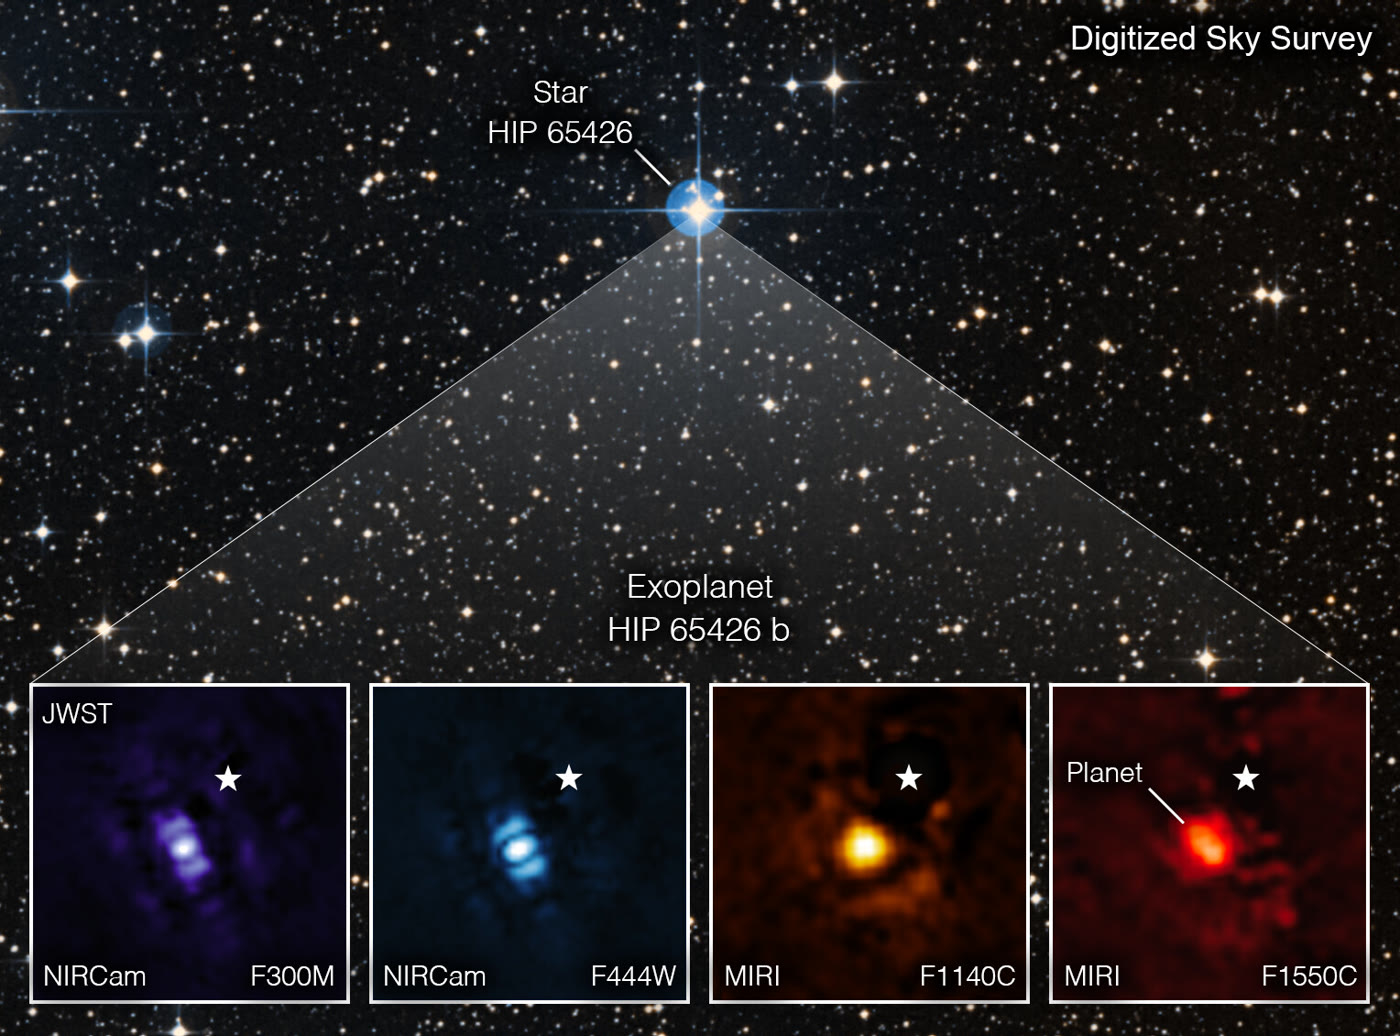
\includegraphics[width=0.86\linewidth]{images/book5/b3-hip65426b.jpg}
\par\smallskip{\small أوّل كوكب خارجي صوّره تلسكوب جيمس ويب
الفضائي، \mbox{\textdir TLT HIP~65426~b}، في أربعة مرشّحات تحت الحمراء (في الأسفل؛ وفي الأعلى،
حقل النجم في مسح سماوي أرضي)؛ ضوء النجم
عند موضع رمز النجم، يُحجب بواسطة
المرقابات الإكليلية. والكوكب عملاق غازي فتيّ كتلته نحو 6 إلى 8
كتل مشترية، وعمره نحو 15 إلى 20 مليون سنة، وهو أبعد عن نجمه بنحو مئة مرّة
مما تبعد الأرض عن الشمس.
الصورة: \mbox{\textdir TLT NASA/ESA/CSA, A~Carter (UCSC), the ERS~1386 team, and A.~Pagan (STScI), CC BY~4.0.}
}\label{fig:b3:exoplanets:hip65426}
\end{omfigure}
% ledger: photo:b3-hip65426b

وتستعمل الطريقة الرابعة الجاذبيةَ عدسةً. فحين يمرّ نجمٌ تقريبًا تمامًا
أمام نجمٍ أبعد، تنحني جاذبيّته ضوءَ النجم
الخلفي ويزيد سطوعه لبضعة أسابيع؛ ويضيف كوكبُ النجم العدسيّ
ومضةً قصيرة.

\begin{definition}[التعديس الجذبوي الصغري؛ نصف قطر أينشتاين]\label{def:b3:exoplanets:microlensing}
\emph{التعديس الجذبوي الصغري}\index{التعديس الجذبوي الصغري} هو
زيادةٌ مؤقتة في سطوع نجمٍ خلفيّ حين يمرّ نجمٌ أماميّ، أي
العدسة، قريبًا من خط النظر؛ والصور التي تكوّنها متقاربةٌ
إلى حدّ لا يمكن معه فصلها. \emph{نصف قطر أينشتاين}\index{نصف قطر أينشتاين}
هو نصف القطر الزاويّ $\theta_\mathrm E$ للحلقة التي تحوّل إليها عدسةٌ نقطية
كتلتها $M$ على البعد $D_L$ مصدرًا على البعد
$D_S$ يقع خلفها تمامًا:
\[
\theta_\mathrm E = \sqrt{\frac{4GM}{c^2}\,\frac{D_S - D_L}{D_L D_S}} .
\]
\end{definition}

\begin{proposition}[تكبير العدسة النقطية]\label{prop:b3:exoplanets:magnification}
مصدرٌ يبعد زاويًّا مقدار $u\,\theta_\mathrm E$ عن عدسة نقطية
يُزاد سطوعه بالعامل
\[
A(u) = \frac{u^2 + 2}{u\sqrt{u^2 + 4}} .
\]
\end{proposition}

\admitted

تنتج النتيجتان كلتاهما عن انحناء الضوء بفعل كتلة ضمن النسبية العامة.
ولعدسة كتلتها نصف كتلة الشمس تقع في منتصف المسافة إلى مصدر
يبعد \qty{8}{kpc}، يكون $\theta_\mathrm E = \qty{0.71}{mas}$، وتكون حلقة
أينشتاين، عند بعد العدسة، نصف قطرها \qty{2.9}{au}. عند
$u = 1$ يزداد سطوع المصدر 1.34 مرة، وعند $u = 0.1$ عشر مرات. كوكبٌ
يقع قرب حلقة أينشتاين لنجمه، فيُضيف انحرافًا قصيرًا إلى
منحنى الضوء. يعثر \omterm{def:b3:exoplanets:microlensing}{التعديس الجذبوي الصغري} إذن على كواكب تبعد بضع وحدات فلكية
عن نجومها، وهي كواكب باردة تُغفلها طريقتا العبور والسرعة الشعاعية،
لكنّ كل حدث يقع مرة واحدة ولا يتكرّر أبدًا. وفي حدث وقع عام 2003،
نُشر في العام التالي، لم يُفسَّر انحراف دام نحو سبعة أيام إلا بمرافق
كتلته $\num{0.0039}$ مرة كتلة العدسة:
كوكب بكتلة نحو 1.5 كتلة المشتري، على بعد نحو \qty{3}{au} من
نجمه.
% ledger: const:G, const:c, sun:mass, iau:parsec, const:au, bond04:ogle235

\begin{omfigure}
\centering
\begin{tikzpicture}[scale=0.95]
\fill (0,0) circle (0.06) node[below=2pt, font=\scriptsize] {المصدر};
\fill[omDef] (3.2,0) circle (0.09); \node[font=\scriptsize, omDef] at (3.2,-1.15) {العدسة};
\draw[omDef] (3.2,0) ellipse (0.12 and 0.9);
\fill (6.4,0) circle (0.06) node[below=2pt, font=\scriptsize] {الراصد};
\draw[thick, orange!80!black] (0,0) -- (3.2,0.9) -- (6.4,0);
\draw[thick, orange!80!black] (0,0) -- (3.2,-0.9) -- (6.4,0);
\draw[densely dashed, black!50] (6.4,0) -- (0,1.8) node[left, font=\scriptsize] {الصورة};
\draw[densely dotted, black!50] (0,0) -- (6.4,0);
\draw[<->] (3.55,0) -- (3.55,0.9) node[midway, right, font=\scriptsize] {$R_\mathrm E$};
\draw[<->, black!60] (0,-1.5) -- (3.2,-1.5) node[midway, below, font=\scriptsize] {$D_S - D_L$};
\draw[<->, black!60] (3.2,-1.5) -- (6.4,-1.5) node[midway, below, font=\scriptsize] {$D_L$};
\end{tikzpicture}\hfill
\begin{tikzpicture}
\begin{axis}[width=0.48\linewidth, height=0.42\linewidth,
  xmin=-3, xmax=3, ymin=0.8, ymax=12, ymode=log,
  ytick={1,2,5,10}, yticklabels={1,2,5,10},
  xlabel={الزمن ($t_\mathrm E$)}, ylabel={التكبير $A$},
  tick label style={font=\scriptsize}, label style={font=\small},
  legend style={font=\scriptsize, at={(0.5,-0.30)}, anchor=north, legend columns=3, draw=none, cells={anchor=west}, /tikz/every even column/.append style={column sep=1em}}]
\addplot[thick, omDef] table[x=t_tE, y=A01] {figdata/out/bachelor-3-rv_transit-lens.dat};
\addlegendentry{$u_0 = 0.1$}
\addplot[thick, dashed, red!70!black] table[x=t_tE, y=A03] {figdata/out/bachelor-3-rv_transit-lens.dat};
\addlegendentry{$0.3$}
\addplot[thick, dotted, black] table[x=t_tE, y=A10] {figdata/out/bachelor-3-rv_transit-lens.dat};
\addlegendentry{$1$}
\end{axis}
\end{tikzpicture}
\par\smallskip{\small يمينًا: هندسة العدسة الثقالية، غير مرسومة
بمقياس؛ تمرّ الأشعة الصادرة عن المصدر بالعدسة عند نحو \omterm{def:b3:exoplanets:microlensing}{نصف قطر أينشتاين}
$R_\mathrm E = \theta_\mathrm E D_L$ ثم تبلغ الراصد الذي يرى
المصدر مُزاحًا إلى الصورة. يسارًا: تكبير مصدر نقطي بعدسة نقطية
بدلالة الزمن، بوحدات الزمن $t_\mathrm E$ الذي تستغرقه العدسة
لتتحرّك مسافة \omterm{def:b3:exoplanets:microlensing}{نصف قطر أينشتاين} واحد، من أجل ثلاث قيم لأقرب اقتراب
$u_0$ (بوحدات \omterm{def:b3:exoplanets:microlensing}{نصف قطر أينشتاين}).}\label{fig:b3:exoplanets:microlensing}
\end{omfigure}

لكلّ طريقةٍ انحيازها الخاص، ويعكس فهرسُ الكواكب المعروفة
هذه الانحيازات. تُفضّل السرعة الشعاعية الكواكب الضخمة القريبة من
نجومها؛ وتُفضّل \omterm{def:b3:exoplanets:transit}{طريقة العبور} الكواكب الكبيرة القريبة من نجومها، وتحتاج إلى
أن يقع المدار في مستوى خط النظر؛ ويعثر \omterm{def:b3:exoplanets:microlensing}{التعديس الجذبوي الصغري} على كواكب
تبعد بضع وحدات فلكية؛ ويعثر \omterm{def:b3:exoplanets:imaging}{التصوير المباشر} على عمالقة شابّة تبعد عشرات أو مئات الوحدات الفلكية.
يُبيّن الشكل أدناه النتيجة: تملأ كل طريقة منطقتها الخاصة،
وتقع معظم كواكب المجموعة الشمسية في الفجوات بينها.

\begin{dated}{2026}
في 23 أكتوبر 2026 أحصى \babelsublr{NASA Exoplanet Archive} 6451 كوكبًا مؤكَّدًا
حسب طريقة الاكتشاف: 4785 بالعبور، 1204 بالسرعة الشعاعية،
292 \omterm{def:b3:exoplanets:microlensing}{بالتعديس الجذبوي الصغري}، 98 \omterm{def:b3:exoplanets:imaging}{بالتصوير المباشر}، 29 \omterm{def:b3:exoplanets:ttv}{بتغيّرات توقيت العبور}، والباقي
بطرائق أندر، ومن بينها أولاها على الإطلاق،
التي عُثر عليها عام 1992 حول نجم نابض بتوقيت نبضاته. وأولى
الاكتشافات بالسرعة الشعاعية تعود إلى عام 1995، وبالعبور إلى عام 2002،
وبالتعديس الجذبوي الصغري \omterm{def:b3:exoplanets:imaging}{والتصوير المباشر} إلى عام 2004.
\end{dated}
% ledger: data:b5-pscomp

\begin{omfigure}
\centering
\begin{tikzpicture}
\begin{axis}[width=0.86\linewidth, height=0.56\linewidth,
  xmode=log, ymode=log, xmin=0.004, xmax=2000, ymin=0.02, ymax=1e5,
  legend image post style={scale=2.2},
  xlabel={نصف المحور الأكبر \babelsublr{(au)}}, ylabel={الكتلة أو الكتلة الدنيا ($M_\oplus$)},
  tick label style={font=\scriptsize}, label style={font=\small},
  legend style={font=\scriptsize, at={(0.5,-0.20)}, anchor=north, legend columns=4, draw=none, cells={anchor=west}, /tikz/every even column/.append style={column sep=1em}}]
\addplot[only marks, mark=*, mark size=0.6pt, omDef, opacity=0.6] table[x=a_au, y=mass] {figdata/out/bachelor-3-exoplanet_archive-ma-tr.dat};
\addlegendentry{العبور}
\addplot[only marks, mark=*, mark size=0.6pt, red!70!black, opacity=0.6] table[x=a_au, y=mass] {figdata/out/bachelor-3-exoplanet_archive-ma-rv.dat};
\addlegendentry{السرعة الشعاعية}
\addplot[only marks, mark=triangle*, mark size=1.2pt, green!45!black] table[x=a_au, y=mass] {figdata/out/bachelor-3-exoplanet_archive-ma-ml.dat};
\addlegendentry{التعديس الجذبوي الصغري}
\addplot[only marks, mark=diamond*, mark size=1.5pt, orange!85!black] table[x=a_au, y=mass] {figdata/out/bachelor-3-exoplanet_archive-ma-im.dat};
\addlegendentry{التصوير المباشر}
\addplot[only marks, mark=square*, mark size=1.6pt, black, forget plot] table[x=a_au, y=mass] {figdata/out/bachelor-3-exoplanet_archive-solar.dat};
\node[font=\scriptsize, anchor=west, fill=white, inner sep=1pt] at (axis cs:1.15,1.0) {الأرض};
\node[font=\scriptsize, anchor=east, fill=white, inner sep=1pt] at (axis cs:0.63,0.82) {الزهرة};
\node[font=\scriptsize, anchor=east, fill=white, inner sep=1pt] at (axis cs:0.34,0.055) {عطارد};
\node[font=\scriptsize, anchor=west, fill=white, inner sep=1pt] at (axis cs:1.75,0.107) {المريخ};
\node[font=\scriptsize, anchor=west, fill=white, inner sep=1pt] at (axis cs:6.0,318) {المشتري};
\node[font=\scriptsize, anchor=west, fill=white, inner sep=1pt] at (axis cs:11,95) {زحل};
\node[font=\scriptsize, anchor=north, fill=white, inner sep=1pt] at (axis cs:25,11) {أورانوس، نبتون};
\end{axis}
\end{tikzpicture}
\par\smallskip{\small كواكب مؤكَّدة ذات كتلة مقيسة (أو \omterm{def:b3:exoplanets:rv}{الكتلة
الدنيا}) ونصف المحور الأكبر، حسب طريقة الاكتشاف (بيانات
\babelsublr{NASA Exoplanet Archive} بتاريخ 23 أكتوبر 2026: 1691 بالعبور، 1151 بالسرعة الشعاعية، 286
\omterm{def:b3:exoplanets:microlensing}{بالتعديس الجذبوي الصغري}، 94 \omterm{def:b3:exoplanets:imaging}{بالتصوير المباشر})، مع كواكب المجموعة الشمسية
(مربعات سوداء). لم تُدرج الكتل المتنبَّأ بها من \omterm{def:b3:exoplanets:mass-radius}{علاقة الكتلة بنصف القطر}. استفاد هذا البحث من
\babelsublr{NASA Exoplanet Archive}، الذي تُشغّله
\babelsublr{California Institute of Technology}، بموجب عقد مع
\babelsublr{National Aeronautics and Space Administration} ضمن
برنامج \babelsublr{Exoplanet Exploration Program}.}\label{fig:b3:exoplanets:methods}
\end{omfigure}
% ledger: data:b5-pscomp, planet:Mercury.mass, planet:Venus.mass, planet:Earth.mass, planet:Mars.mass, planet:Jupiter.mass, planet:Saturn.mass, planet:Uranus.mass, planet:Neptune.mass, planet:Mercury.dist, planet:Venus.dist, planet:Earth.dist, planet:Mars.dist, planet:Jupiter.dist, planet:Saturn.dist, planet:Uranus.dist, planet:Neptune.dist

\section{ما الذي وُجد}\label{sec:b3:exoplanets:found}

كانت أولى المفاجآت هي المشتريات الحارة، وهي كواكب عملاقة على مدارات تبلغ
بضعة أيام. لا يمكن أن يكون 51~بيغاسي~b قد تشكّل قريبًا إلى هذا الحد من نجمه؛ بل لا بدّ أنّه
تشكّل أبعد، ربما على بُعد بضع وحدات فلكية، خارج
خطّ الثلج في قرصه، وهاجر نحو الداخل عبر تفاعله مع القرص،
كما تنبّأت النظرية بذلك.
% ledger: nobel19:migration

\begin{definition}[المشتري الحار؛ الأرض الفائقة؛ ما دون نبتون]\label{def:b3:exoplanets:classes}
\emph{المشتري الحار}\index{المشتري الحار} هو كوكب عملاق على مدار قريب،
ويُعدّ عادةً ذا كتلة دنيا تزيد على 0.1 من كتلة المشتري ودورٍ
أقصر من عشرة أيام. أمّا \emph{الأرض الفائقة}\index{الأرض الفائقة} فهي كوكب
أكبر من الأرض لكنّها أصغر من \omterm{def:b3:exoplanets:radius-valley}{وادي نصف القطر}، أي حتى نحو
1.5 إلى 2 من أنصاف أقطار الأرض، ومن ثمّ يُرجَّح أنّها صخرية. أمّا \emph{ما دون نبتون}\index{ما دون نبتون}
فهو كوكب يعلو \omterm{def:b3:exoplanets:radius-valley}{وادي نصف القطر} لكنّه أصغر من نبتون، ويبلغ نحو 2 إلى
4 من أنصاف أقطار الأرض، ويتطلّب نصف قطره غلافًا من الغازات الخفيفة أو
المواد المتطايرة.
\end{definition}
% ledger: wright12:hj, fulton17:gap, planet:Neptune.diameter, planet:Earth.diameter

\begin{definition}[معدّل الوقوع]\label{def:b3:exoplanets:occurrence}
\emph{معدّل الوقوع}\index{معدّل الوقوع} لفئة من الكواكب هو
متوسط عدد هذه الكواكب لكلّ نجم، أو نسبة النجوم التي
تستضيف واحدًا منها، ضمن مدى معيّن من الحجم (أو الكتلة) والدور، بعد
تصحيح أعداد المسح للكواكب التي لم يتمكّن من رصدها:
أي تلك التي لا تكون مداراتها مصطفّة للعبور، والتي تكون صغيرة جدًّا أو
بعيدة جدًّا بحيث لا تُرى.
\end{definition}

المشتريات الحارة، وهي بارزة في الفهرس لأنّها الأسهل رصدًا، نادرة:
فقد وجد مسح \omterm{def:b3:exoplanets:rv}{بطريقة السرعة الشعاعية} لنجوم قريبة شبيهة بالشمس أنّها تحيط بنحو
\qty[separate-uncertainty=true]{1.2 \pm 0.38}{\percent} من النجوم. والكواكب الصغيرة شائعة.
وفي بحث أُجري على منحنيات ضوء \num{42000} نجم رصدها تلسكوب الفضاء كبلر،
عثرت دراسة واحدة على 603 كواكب، منها عشرة بحجم الأرض (من 1 إلى 2
من أنصاف أقطار الأرض)، وتتلقّى ما بين مرّة وأربع مرّات ما تتلقّاه الأرض
من ضوء الشمس؛ وبعد تصحيح احتمال العبور والكواكب التي كان البحث سيُفوّتها،
\qty[separate-uncertainty=true]{11 \pm 4}{\percent} من النجوم الشبيهة بالشمس تستضيف
كوكبًا من هذا النوع.
% ledger: wright12:hj, petigura13:eta

ولا تتوزّع أحجام الكواكب الصغيرة توزّعًا متساويًا. فمن بين الكواكب القريبة
التي قيست بدقّة، فإنّ التي يتراوح نصف قطرها بين 1.5 و2.0 من أنصاف أقطار الأرض تكون أندر بمرّتين على الأقل
من تلك التي تقلّ عنها أو تزيد عليها بقليل.

\begin{definition}[وادي نصف القطر]\label{def:b3:exoplanets:radius-valley}
\emph{وادي نصف القطر}\index{وادي نصف القطر} هو نقص الكواكب
التي يتراوح أنصاف أقطارها بين نحو 1.5 و2.0 من أنصاف أقطار الأرض، ضمن الكواكب
التي تقلّ أدوارها عن نحو مائة يوم؛ وهو يفصل \omterm{def:b3:exoplanets:classes}{الأرض الفائقة}
عن كواكب \omterm{def:b3:exoplanets:classes}{ما دون نبتون}.
\end{definition}
% ledger: fulton17:gap

يُقرأ الوادي بوصفه أثرًا للإفلات. فاللبّ الصخري الذي يتشكّل ومعه غلاف
من الهيدروجين والهليوم لا تتجاوز بضعة في المئة من كتلته، يبلغ نصف قطره ضعف نصف قطر اللبّ المجرّد.
وبالقرب من نجم فتيّ نشط، يُسخَّن ذلك الغلاف ويُفقد
\omterm{def:b3:planetary-atmospheres:hydrodynamic}{بالإفلات الهيدروديناميكي}: بفعل إشعاع النجم عالي الطاقة خلال
أوّل مائة مليون سنة (التبخّر الضوئي)، أو بحرارة اللبّ المتبرّد نفسه
(فقدان الكتلة
بطاقة اللبّ). وتدفع النماذج الكواكب إلى لبّ مجرّد نصف قطره نحو 1.3 من أنصاف أقطار الأرض،
وكواكب بضعف ذلك الحجم؛ ولا يبقى إلّا القليل بينهما. وتعتمد الآليتان
على النجم اعتمادًا مختلفًا، والكواكب التي تدور حول نجوم من أنواع
مختلفة قد تُمكّن من التمييز بينهما.
% ledger: owen17:valley, ginzburg18:core-powered

\begin{omfigure}
\centering
\begin{tikzpicture}
\begin{axis}[name=pr, width=0.50\linewidth, height=0.50\linewidth,
  xmode=log, ymode=log, xmin=1, xmax=100, ymin=0.8, ymax=4,
  ytick={1,1.5,2,3,4}, yticklabels={1,1.5,2,3,4},
  xlabel={الدور (بالأيام)}, ylabel={نصف القطر ($R_\oplus$)},
  tick label style={font=\scriptsize}, label style={font=\small},
  title={(أ)}, title style={font=\small}]
\fill[black!10] (axis cs:1,1.5) rectangle (axis cs:100,2.0);
\addplot[only marks, mark=*, mark size=0.5pt, omDef, opacity=0.7] table[x=period, y=radius] {figdata/out/bachelor-3-exoplanet_archive-pr.dat};
\end{axis}
\begin{axis}[at={(pr.east)}, anchor=west, xshift=0.09\linewidth,
  width=0.42\linewidth, height=0.50\linewidth,
  xmode=log, xmin=0.8, xmax=4, ymin=0, ymax=185,
  xtick={1,1.5,2,3,4}, xticklabels={1,1.5,2,3,4},
  xlabel={نصف القطر ($R_\oplus$)}, ylabel={عدد الكواكب},
  tick label style={font=\scriptsize}, label style={font=\small},
  title={(ب)}, title style={font=\small}]
\fill[black!10] (axis cs:1.5,0) rectangle (axis cs:2.0,185);
\addplot[const plot mark left, thick, omDef, fill=omDef!25] table[x=r, y=n] {figdata/out/bachelor-3-exoplanet_archive-histstep.dat} \closedcycle;
\end{axis}
\end{tikzpicture}
\par\smallskip{\small (أ)~كواكب عابرة ذات أنصاف أقطار معروفة بدقّة أفضل من
\qty{10}{\percent}، حول نجوم أصغر من نصفي قطر شمسي، ذات أدوار
من 1 إلى 100 يومًا (عدد الكواكب 2370، \babelsublr{NASA Exoplanet Archive}، 23
أكتوبر 2026)؛ المظلّل هو \omterm{def:b3:exoplanets:radius-valley}{وادي نصف القطر} البالغ 1.5 إلى 2.0 من أنصاف أقطار الأرض.
(ب)~الكواكب نفسها معدودة في 20 فئة متساوية العرض بمقياس $\log R$.
ولم تُصحَّح الأعداد لتشمل الكواكب التي تفوّتها المسوح، وهي
أكثر عددًا بين الصغيرة منها؛ ومع ذلك يظهر الوادي.}\label{fig:b3:exoplanets:valley}
\end{omfigure}
% ledger: data:b5-pscomp, fulton17:gap

\begin{definition}[علاقة الكتلة بنصف القطر]\label{def:b3:exoplanets:mass-radius}
\emph{علاقة الكتلة بنصف القطر}\index{علاقة الكتلة بنصف القطر} لتركيبٍ ما
هي نصف قطر كوكب ذي ذلك التركيب بوصفه دالّةً لكتلته،
محسوبًا من معادلات الحالة لموادّه
في التوازن الهيدروستاتيكي؛ ويُقارَن الكوكب المقيس مع
علاقات التراكيب المرشّحة.
\end{definition}

يُضغط الكوكب الصخري بوزنه الذاتي، ويتزايد نصف قطره
أبطأ من $M^{1/3}$. وقد أُجريت ملاءمة لنماذج كواكب ذات طبقتين مبنية على
النموذج الزلزالي للأرض، فأعطت العلاقة $R/R_\oplus = (1.07 - 0.21\,C)
(M/M_\oplus)^{1/3.7}$، من أجل 1 إلى 8 من كتل الأرض، ونسبة كتلة اللبّ
$C$ من 0 إلى 0.4؛ وعند ملاءمتها للأرض والزهرة وعدد من الكواكب الخارجية
الصغيرة، تُعطي $C = 0.26 \pm 0.07$. أمّا
كوكب الحديد فيكون أصغر عند الكتلة نفسها؛ وكوكب نصفه ماء أكبر؛
وغلاف من الهيدروجين لا تتجاوز نسبته اثنين في المئة من الكتلة يجعل الكوكب ذا
خمس كتل أرضية ونصف قطر \num{2.6} من أنصاف أقطار الأرض، أي بحجم
\omterm{def:b3:exoplanets:classes}{ما دون نبتون}. والتنكّس حقيقي: فنصف القطر والكتلة يُعطيان كثافة واحدة، ويمكن
لعدّة خلائط من الحديد والصخر والماء والغاز أن تشترك فيها.
فالكوكب الصخري كبلر-10~b، الذي كتلته 3.24 من كتل الأرض ونصف قطره 1.47 من أنصاف أقطار الأرض،
له متوسط كثافة \qty{5.6}{g.cm^{-3}}؛ أمّا العملاق الغازي واسب-39~b،
الذي كتلته 89 من كتل الأرض ونصف قطره 14.3 من أنصاف أقطار الأرض، فكثافته \qty{0.17}{g.cm^{-3}}.
% ledger: zeng16:rocky, data:b5-zeng, data:b5-pscomp

\begin{omfigure}
\centering
\begin{tikzpicture}
\begin{axis}[width=0.86\linewidth, height=0.58\linewidth,
  xmode=log, ymode=log, xmin=0.3, xmax=5000, ymin=0.5, ymax=25,
  ytick={0.5,1,2,4,10,20}, yticklabels={0.5,1,2,4,10,20},
  xlabel={الكتلة ($M_\oplus$)}, ylabel={نصف القطر ($R_\oplus$)},
  tick label style={font=\scriptsize}, label style={font=\small},
  legend style={font=\scriptsize, at={(0.5,-0.20)}, anchor=north, legend columns=3, draw=none, cells={anchor=west}, /tikz/every even column/.append style={column sep=1em}}]
\addplot[only marks, mark=*, mark size=0.6pt, black!35, forget plot] table[x=mass, y=radius] {figdata/out/bachelor-3-exoplanet_archive-mr.dat};
\addplot[thick, black] table[x=mass, y=radius] {figdata/out/bachelor-3-exoplanet_archive-zeng-iron.dat};
\addlegendentry{الحديد النقي}
\addplot[thick, brown!70!black] table[x=mass, y=radius] {figdata/out/bachelor-3-exoplanet_archive-zeng-earthlike.dat};
\addlegendentry{صخر شبيه بالأرض}
\addplot[thick, omDef] table[x=mass, y=radius] {figdata/out/bachelor-3-exoplanet_archive-zeng-water50.dat};
\addlegendentry{\foreignlanguage{arabic}{\mbox{\textdir TLT 50\,\%} ماء}}
\addplot[thick, dashed, orange!85!black] table[x=mass, y=radius] {figdata/out/bachelor-3-exoplanet_archive-zeng-h2-2pc.dat};
\addlegendentry{\foreignlanguage{arabic}{صخر + 2\,\% هيدروجين}}
\addplot[only marks, mark=square*, mark size=1.8pt, red!70!black] table[x=mass, y=radius] {figdata/out/bachelor-3-exoplanet_archive-solar.dat};
\addlegendentry{النظام الشمسي}
\node[font=\scriptsize, anchor=north west] at (axis cs:1.05,0.97) {الأرض};
\node[font=\scriptsize, anchor=south east] at (axis cs:0.80,0.97) {الزهرة};
\node[font=\scriptsize, anchor=south east, fill=white, inner sep=1pt] at (axis cs:13.5,4.3) {أورانوس، نبتون};
\node[font=\scriptsize, anchor=east, fill=white, inner sep=1pt] at (axis cs:80,9.45) {زحل};
\node[font=\scriptsize, anchor=north, fill=white, inner sep=1pt] at (axis cs:318,10.3) {المشتري};
\end{axis}
\end{tikzpicture}
\par\smallskip{\small كتلة ونصف قطر 1078 كوكبًا عابرًا تُقاس كتلته
بدقّة أفضل من \qty{25}{\percent}، ونصف قطره بدقّة أفضل من
\qty{10}{\percent} (باللون الرمادي؛ \babelsublr{NASA Exoplanet Archive}، 23 أكتوبر 2026)،
مع منحنيات نموذجية لزينغ وآخرين (2016، 2019): الحديد النقي؛
الصخر الشبيه بالأرض، ثلثه حديد وثلثاه سيليكات؛ ونصف ماء على مثل هذا
اللبّ، عند \qty{500}{K}؛ ولبٌّ شبيه بالأرض مع غلاف من الهيدروجين بنسبة
\qty{2}{\percent} من كتلته، عند \qty{500}{K}. المربّعات الحمراء: كواكب
النظام الشمسي (يقع عطارد والمرّيخ خارج المقياس، نحو
اليسار).}\label{fig:b3:exoplanets:mass-radius}
\end{omfigure}
% ledger: data:b5-pscomp, data:b5-zeng, planet:Earth.mass, planet:Earth.diameter, planet:Venus.mass, planet:Venus.diameter, planet:Jupiter.mass, planet:Jupiter.diameter, planet:Saturn.mass, planet:Saturn.diameter, planet:Uranus.mass, planet:Uranus.diameter, planet:Neptune.mass, planet:Neptune.diameter

\section{الأغلفة الجوية}\label{sec:b3:exoplanets:atmospheres}

يمكن وزن الكوكب العابر وقياسه؛ ويمكن كذلك شمّه.
أثناء العبور، تقع أمام النجم حلقة رقيقة من الغلاف الجوي للكوكب،
فيتسرّب ضوء النجم عبرها. وعند الأطوال الموجية التي يمتصّ فيها غازٌ
من الغلاف الجوي، تصبح الحلقة معتمةً في الارتفاعات الأعلى، فيبدو الكوكب
أكبر حجمًا.

\begin{definition}[مطيافية النفاذ؛ الكسوف الثانوي]\label{def:b3:exoplanets:transmission}
\emph{مطيافية النفاذ}\index{مطيافية النفاذ} تقيس \omterm{def:b3:exoplanets:transit}{عمق العبور} بدلالة طول الموجة،
للكشف عن غازات الغلاف الجوي التي يعبرها ضوء النجم عند
حافة الكوكب.
\emph{الكسوف الثانوي}\index{الكسوف الثانوي} هو مرور
الكوكب خلف نجمه، بعد نصف دورة مدارية من العبور في مدار دائري؛
فإنّ انخفاض تدفّق النظام عندئذٍ يقيس ضوء
الجانب النهاري للكوكب.
\end{definition}

\begin{proposition}[إشارة النفاذ]\label{prop:b3:exoplanets:transmission}
غلافٌ جوي ذو ارتفاع مقياسي $H \ll R_p$، يُجعل معتمًا عبر $n$ ارتفاعًا مقياسيًا إضافيًا
عند طول موجة نطاق امتصاص، مقارنةً بالأطوال الموجية المجاورة،
يُعمِّق العبور هناك بمقدار
\[
\Delta\delta \approx n\,\frac{2HR_p}{R_\star^2} .
\]
\end{proposition}

\begin{proof}
يزداد نصف القطر الظاهري للكوكب من $R_p$ إلى $R_p + nH$، فإنّ
يزداد العمق $(R_p + nH)^2/R_\star^2$ بمقدار $(2nHR_p + n^2H^2)/R_\star^2$،
وهو $2nHR_p/R_\star^2$ عندما يكون $nH \ll R_p$.
\end{proof}

الارتفاع المقياسي $H = kT/\bar m g$ كبيرٌ في كوكب حارّ منخفض الجاذبية
يحوي هواءً خفيفًا من الهيدروجين، وصغيرٌ في كوكب بارد كثيف يحوي
هواءً ثقيلًا. ومن أجل الأرض مرصودةً على خلفية الشمس، مع $H = \qty{8}{km}$،
يُضيف كل ارتفاع مقياسي 0.2 جزء في المليون؛ وفي عملاق غازي حارّ منتفخ،
عدّة مئات.
% ledger: planet:Earth.diameter, sun:R

\begin{proposition}[عمق الكسوف الثانوي]\label{prop:b3:exoplanets:eclipse}
إذا كان الجانب النهاري لكوكب يشعّ كجسم أسود عند الدرجة
$T_d$ ويشعّ النجم كجسم أسود عند $T_\star$، فإنّ \omterm{def:b3:exoplanets:transmission}{الكسوف الثانوي} عند الطول الموجي
$\lambda$ يكون عمقه
\[
\delta_\mathrm{ecl} \approx \left(\frac{R_p}{R_\star}\right)^2
  \frac{B_\lambda(T_d)}{B_\lambda(T_\star)},
\]
حيث $B_\lambda$ قانون بلانك، مع إهمال الضوء المنعكس عن الكوكب.
\end{proposition}

\begin{proof}
قبيل الكسوف يستقبل الراصد ضوء النجم، متناسبًا مع
$\pi R_\star^2 B_\lambda(T_\star)$، مضافًا إليه ضوء الجانب النهاري،
متناسبًا مع $\pi R_p^2 B_\lambda(T_d)$؛ وأثناء الكسوف لا يبقى سوى
ضوء النجم. والانخفاض الكسري هو نسبة حدّ الكوكب إلى حدّ النجم،
إذ إنّ حدّ الكوكب صغير.
\end{proof}

يكون الكسوف أعمق ما يكون في الأشعة تحت الحمراء، حيث يكون الكوكب البارد
أكثر إشراقًا بالنسبة إلى نجمه: فهو يعطي درجة حرارة الجانب النهاري.
ويكشف جانب نهاري حارّ مجاور لجانب ليلي بارد عن غلاف جوي رقيق أو غائب
لا يوزّع الحرارة.

\begin{dated}{2023}
في عام 2022 أظهر طيف النفاذ للعملاق الغازي واسب-39~b، الذي قيس
بين 3.0 و\qty{5.5}{\micro m} بواسطة تلسكوب جيمس ويب الفضائي،
أظهر نطاق امتصاص بارزًا لثاني أكسيد الكربون عند
\qty{4.3}{\micro m}، بمقدار 26 انحرافًا معياريًا، حيث لم تكن القياسات الضوئية السابقة قد أشارت إليه إلّا
تلميحًا: وكان ذلك أوّل تحديدٍ واضح له
في غلاف جوي لكوكب خارجي. وفي عام 2023 قيست خمسة كسوفات ثانوية
للكوكب ترابيست-1~b بحجم الأرض، الذي يتلقّى أربعة أضعاف ما تتلقّاه الأرض من ضوء الشمس
من نجمٍ بارد صغير، وقيست عند \qty{15}{\micro m}. وهي تتوافق
مع حرارة معاد إشعاعها من الجانب النهاري وحده، دون ثاني أكسيد كربون قابل للكشف:
فالكوكب لا يملك غلافًا جويًا يُذكر، أو يملك القليل منه، لينقل الحرارة
إلى جانبه الليلي.
\end{dated}
% ledger: jwst23:wasp39-co2, greene23:trappist1b

الكواكب الصخرية في النطاقات الصالحة للحياة حول النجوم الصغيرة في متناول هذه الطرق
لكن على الحدّ الأقصى لقدرتها. وهل احتفظت بغلافها الجوي أمام عمليات
الإفلات التي تناولها الفصل السابق، فهذا الآن سؤال رصدي
مطروح للرصد.

\section{التمارين}

\begin{exercise}[$\star$]\label{exo:b3:exoplanets:1}
(أ)~احسب السعة النصفية للسرعة الشعاعية للشمس الناتجة عن
المشتري (الكتلة \qty{1898e24}{kg}، الدور \num{4331}~يومًا، اللامركزية
0.049) والناتجة عن الأرض (الكتلة \qty{5.97e24}{kg}، الدور \num{365.2}~يومًا،
اللامركزية 0.017). وكتلة الشمس \qty{1.9884e30}{kg}.
(ب)~حوّل الدقّتين \qty{3.5}{km/h} و\qty{0.35}{km/h} إلى
أمتار في الثانية، وقارن النتيجتين.
\end{exercise}

\begin{exercise}[$\star$]\label{exo:b3:exoplanets:2}
(أ)~احسب عمقي العبور للمشتري (نصف القطر \qty{71492}{km})
وللأرض (نصف القطر \qty{6378}{km}) عبر الشمس (نصف القطر
\qty{695700}{km}). (ب)~احسب احتمال أن يرى مراقب موضوع عشوائيًا
كلًّا منهما يعبر، عند أنصاف أقطار مدارية تبلغ \num{778.5}
و\qty{149.6}{\mega km}.
\end{exercise}

\begin{exercise}[$\star$]\label{exo:b3:exoplanets:3}
تُنتج 51~بيغاسي~b في نجمها سعةً نصفيةً للسرعة الشعاعية مقدارها
\qty{59}{m.s^{-1}}، ودوره \qty{4.23}{d}. وبأخذ كتلة النجم مساوية لكتلة الشمس،
احسب \omterm{def:b3:exoplanets:rv}{الكتلة الدنيا} للكوكب بوحدات كتلة المشتري
وبوحدات كتلة الأرض، ونصف قطر مداره.
\end{exercise}

\begin{exercise}[$\star$]\label{exo:b3:exoplanets:4}
نجم كتلته نصف كتلة الشمس على بعد \qty{4}{kpc} يُعدِّس نجمًا يقع على بعد
\qty{8}{kpc} ($\qty{1}{pc} = \qty{3.0857e16}{m}$). (أ)~احسب
\omterm{def:b3:exoplanets:microlensing}{نصف قطر أينشتاين} للعدسة بالميلي ثانية قوسية، ونصف قطر حلقة أينشتاين،
بالوحدات الفلكية، عند بعد العدسة. (ب)~احسب
التكبير عند $u = 1$، و$0.5$، و$0.1$. (ج)~كم يستغرق مرور العدسة
لعبور \omterm{def:b3:exoplanets:microlensing}{نصف قطر أينشتاين} الواحد إذا كانت تتحرك عبر خط النظر بسرعة
\qty{200}{km.s^{-1}}؟
\end{exercise}

\begin{exercise}[$\star\star$]\label{exo:b3:exoplanets:5}
كوكب نسبة نصفي قطره $p = 0.12$ يدور حول نجم كتلته كتلة شمسية واحدة
ونصف قطره نصف قطر شمسي واحد، في \qty{3.0}{d}. (أ)~احسب $a/R_\star$. (ب)~احسب
$T_{14}$ و$T_{23}$ من أجل $b = 0$ ومن أجل $b = 0.7$، وميل المدار
في الحالة الثانية. (ج)~كيف يميّز شكل المنحنى الضوئي عبورًا مركزيًّا من عبور
مماسّي؟
\end{exercise}

\begin{exercise}[$\star\star$]\label{exo:b3:exoplanets:6}
من الكتل وأنصاف الأقطار في \babelsublr{Exoplanet Archive}، احسب متوسطات
كثافات ترابيست-1~b (1.374 كتلة أرضية، و1.116 نصف قطر أرضي)،
كبلر-10~b (3.24، 1.47)، واسب-39~b (89.31، 14.34)، و\babelsublr{HD~209458~b} (232.0،
15.58)، مع $M_\oplus = \qty{5.97e24}{kg}$ و$R_\oplus =
\qty{6378}{km}$. أيّها صخرية وأيّها غازية؟
\end{exercise}

\begin{exercise}[$\star\star$]\label{exo:b3:exoplanets:7}
السرعة الشعاعية لنجم يدور حوله كوكب واحد على مدار لامركزي
تتراوح من $+\qty{50.4}{m.s^{-1}}$ إلى $-\qty{9.6}{m.s^{-1}}$، وسرعة
مركز كتلة المنظومة \qty{12.4}{m.s^{-1}}. مستعينًا بالصيغة
اللامركزية للمبرهنة، احسب $K$ و$e\cos\omega$. لماذا يمكن أن يختلف
متوسط القيمتين المتطرفتين عن $\gamma$؟
\end{exercise}

\begin{exercise}[$\star\star$]\label{exo:b3:exoplanets:8}
واسب-39~b له 89.31 كتلة أرضية و14.34 نصف قطر أرضي؛ ونجمه 0.939
نصف قطر شمسي. خذ درجة حرارة \qty{1100}{K} ومتوسط الكتلة الجزيئية
\qty{2.3}{u} لغلافه الجوي. (أ)~احسب جاذبيته، وارتفاع
ارتفاع المقياس وعمق عبوره. (ب)~احسب إشارة النفاذ لارتفاع مقياسي واحد،
ولحزمة امتصاص ارتفاعها مقياسان، بالأجزاء
في المليون.
\end{exercise}

\begin{exercise}[$\star\star$]\label{exo:b3:exoplanets:9}
ترابيست-1~b له نصف قطر 1.116 نصف قطر أرضي؛ ونجمه 0.1192 نصف قطر شمسي
و\qty{2566}{K}. احسب عمق كسوفه الثانوي عند
\qty{15}{\micro m} لجانب نهاري عند \qty{400}{K} وعند \qty{500}{K}
($hc/k = \qty{0.014388}{m.K}$). لماذا يُعدّ قياس العمق
مقياسَ حرارة؟
\end{exercise}

\begin{exercise}[$\star\star\star$]\label{exo:b3:exoplanets:10}
قزم أحمر متخيّل له 0.2 كتلة شمسية، و0.2 نصف قطر شمسي،
وإشعاعية تبلغ \num{0.005} من الإشعاعية الشمسية. (أ)~على أيّ بعد يتلقّى كوكب
الدفق النجمي الذي تتلقّاه الأرض، وما دوره؟
(ب)~احسب السعة النصفية الناجمة عن كوكب كتلته كتلة أرضية واحدة
هناك، وقارنها بتأثير الأرض في الشمس. (ج)~احسب
\omterm{def:b3:exoplanets:transit}{عمق العبور} لكوكب بحجم الأرض. لماذا تكون هذه النجوم مفضّلة
أهدافًا في البحث عن الكواكب الصخرية في النطاقات الصالحة للحياة؟
\end{exercise}

\begin{exercise}[$\star\star\star$]\label{exo:b3:exoplanets:11}
بالنسبة لقانون \omterm{def:b3:exoplanets:limb}{إعتام الحافة} التربيعي، بيّن أنّ متوسط شدة
القرص هو $I(1)(1 - u_1/3 - u_2/6)$. استنتج العمق، بوحدات
$p^2$، لكوكب صغير عند $r = 0$، و$0.5$، و$0.9$ من أجل $u_1 = 0.40$،
$u_2 = 0.25$. أيّ خطأ يرتكبه نموذج القرص المتجانس في نصف قطر
كوكب يُرصد عند منتصف العبور حين $b = 0$؟
\end{exercise}

\begin{exercise}[$\star\star\star$]\label{exo:b3:exoplanets:12}
رصدت دراسة مسحية \num{42000} نجم شبيه بالشمس، وبحثت فيها عن
كواكب بحجم الأرض تتلقّى من ضوء الشمس بين مرّة وأربع مرات ما تتلقّاه الأرض،
أي في مدارات من 0.5 إلى \qty{1}{au}. (أ)~احسب احتمال العبور
عند 0.5 و0.7 و\qty{1}{au}. (ب)~إذا كانت \qty{11}{\percent} من
النجوم تستضيف كوكبًا من هذا النوع، عند نحو \qty{0.7}{au}، فكم منها يعبر؟
(ج)~وجدت الدراسة عشرة. ماذا يقيس الفرق، ولماذا يجب
تصحيح \omterm{def:b3:exoplanets:occurrence}{معدّل الوقوع} لأجله؟
\end{exercise}

\section{مسألة: كوكب حول مصباح سيلين}

\begin{problem}[{مسألة نهاية الأسبوع --- وزن كوكب
مُختلَق وقياس حجمه وتحليل غلافه الجوي}]
\label{pb:b3:exoplanets:1}
مصباح سيلين قزم K مُختلَق كتلته 0.80 كتلة شمسية، ونصف قطره
0.76 نصف قطر شمسي ودرجة حرارته الفعّالة \qty{5000}{K}. مسحٌ
\omterm{def:b3:exoplanets:rv}{بطريقة السرعة الشعاعية} يجد أنّ سرعته تتغيّر جيبيًا مع
دورٍ قدره \qty{12.0}{d} ونصف سعة \qty{2.59}{m.s^{-1}}. وبعد
ذلك يرصد تلسكوب فضائي عبورات بالدور نفسه، بعمق
\num{838} جزءًا في المليون ومدة كلية $T_{14} = \qty{3.23}{h}$.
خذ $M_\odot = \qty{1.9884e30}{kg}$، $R_\odot = \qty{695700}{km}$،
$L_\odot = \qty{3.828e26}{W}$, $M_\oplus = \qty{5.97e24}{kg}$,
$R_\oplus = \qty{6378}{km}$.

\medskip\noindent\textbf{الجزء الأول --- السرعة الشعاعية.}
\begin{enumerate}
\item احسب نصف قطر المدار، بالأمتار وبالوحدات الفلكية
  مُهمِلًا كتلة الكوكب بالنسبة إلى كتلة النجم.
\item احسب السرعة المدارية للكوكب.
\item احسب \omterm{def:b3:exoplanets:rv}{الكتلة الدنيا} للكوكب، بوحدات كتلة الأرض.
\item احسب نصف قطر مدار النجم نفسه حول مركز
  الكتلة، وتحقّق من أنّه يعطي نصف السعة المرصود.
\item بكم مرّة تتجاوز الإشارة دقّة
  \qty{1}{m.s^{-1}}، و\qty{0.1}{m.s^{-1}}؟
\item لو كان للمدار $e = 0.2$ مع بقاء $K$ نفسه، فما مقدار
  التغيّر في \omterm{def:b3:exoplanets:rv}{الكتلة الدنيا}؟
\end{enumerate}

\medskip\noindent\textbf{الجزء الثاني --- العبور.}
\begin{enumerate}[resume]
\item احسب نسبة نصفي القطرين $p = R_p/R_\star$.
\item احسب نصف قطر الكوكب بالكيلومترات وبوحدات نصف قطر الأرض.
\item احسب $a/R_\star$.
\item احسب مدة العبور المركزي ($b = 0$).
\item انطلاقًا من $T_{14}$ المرصود، احسب \omterm{def:b3:exoplanets:transit}{معامل التصادم}.
\item احسب ميل المدار.
\item ما كان احتمال أن يعبر هذا الكوكب، منظورًا إليه من
  اتجاه عشوائي؟
\end{enumerate}

\medskip\noindent\textbf{الجزء الثالث --- ممَّ يتكوّن؟}
\begin{enumerate}[resume]
\item احسب الكتلة الحقيقية للكوكب.
\item احسب متوسط كثافته.
\item على منحنى النموذج الصخري الشبيه بالأرض، يُتوقّع لكوكب بهذه الكتلة
  أن يكون له نصف قطر قدره 1.74 من أنصاف أقطار الأرض. قارن، واذكر ما يجب أن يحتويه
  الكوكب فضلًا عن الصخر.
\item أين يقع الكوكب بالنسبة إلى \omterm{def:b3:exoplanets:radius-valley}{وادي نصف القطر}؟ هل هو
  \omterm{def:b3:exoplanets:classes}{الأرض الفائقة} أم \omterm{def:b3:exoplanets:classes}{ما دون نبتون}؟
\item احسب جاذبية سطحه.
\end{enumerate}

\medskip\noindent\textbf{الجزء الرابع --- غلافه الجوي.}
\begin{enumerate}[resume]
\item احسب إشعاعية النجم بالواط وبوحدات الإشعاعية
  الشمسية.
\item احسب الدفق النجمي الذي يتلقّاه الكوكب، نسبةً إلى
  الأرض. هل يقع في النطاق الصالح للحياة؟
\item بافتراض ألبيدو بوند يساوي 0.3، احسب درجة حرارة توازنه.
\item احسب ارتفاع المقياس لغلاف جوّي من الهيدروجين والهليوم
  (متوسط الكتلة الجزيئية \qty{2.3}{u}) عند تلك الدرجة الحرارة.
\item احسب إشارة النفاذ لارتفاع مقياس واحد، ولشريط
  امتصاص مائي بارتفاع مقياسين، بالأجزاء في المليون.
\item احسب الكمية نفسها لغلاف جوي من بخار الماء (\qty{18}{u}). أيّ من
  الغلافين يستطيع تلسكوب فضائي بدقّة نحو عشرة أجزاء في المليون
  أن يميّزه عن طيف مستوٍ؟
\item أعطِ متوسط كثافة الكوكب، بالغرام لكل سنتيمتر مكعّب، إلى
  رقمين معنويين.
\end{enumerate}
\end{problem}
% ledger: sun:mass, sun:R, sun:L, planet:Earth.mass, planet:Earth.diameter, const:G, const:kB, const:sigma, nist:u, data:b5-zeng, fulton17:gap, eso:espresso
